\chapter{आणविक विकास और जातिवृत्तजीनोमिकी}\label{ch:b3:molecular-evolution}

1968 में मोतू किमूरा ने कोई ऐसा जोड़ किया जिसने एक पूरे क्षेत्र को हिला
दिया। उन स्तनियों के हीमोग्लोबिन, साइटोक्रोम और दूसरे प्रोटीन, जिनके
साझा पूर्वजों की तिथियाँ जीवाश्मों से तय थीं, आपस में मिलाकर उसने पाया
कि ऐमीनो अम्ल मोटे तौर पर प्रति स्थल प्रति अरब वर्ष एक प्रतिस्थापन की
दर से बदले हैं --- जो, किसी स्तनी जीनोम और किसी पीढ़ी भर में, लगभग हर दो
वर्ष में उस समष्टि में स्थिर हुए किसी नए प्रतिस्थापन तक पहुँचता था।
हाल्डेन ने दशक भर पहले दिखाया था कि प्राकृतिक वरण, इससे पहले कि खोई
संतति की लागत अदेय हो जाए, अधिक से अधिक तीन सौ पीढ़ियों में लगभग एक
प्रतिस्थापन स्थिर कर सकता है। उस अंकगणित ने एक ही रास्ता छोड़ा:
DNA में जमा होने वाले अधिकांश बदलाव वरण से चलते ही नहीं, बल्कि उदासीन
हैं, जो परिमित समष्टियों में संयोग से स्थिर होते हैं, और वह भी ऐसी दर
से जो --- जैसा इस अध्याय का पहला प्रमेय दिखाता है --- बस उत्परिवर्तन-दर
है। \omterm{thm:b3:molecular-evolution:neutral}{उदासीन सिद्धांत} आणविक विकास की निराकरणीय परिकल्पना बन गया, यानी वह
आधार-रेखा जिसके सामने वरण पकड़ा जाता है; \omterm{prop:b3:molecular-evolution:clock}{आणविक घड़ी} उसकी तिथियाँ निकालने
का कोई ढंग बन गई जो जीवाश्म नहीं निकाल सकते; और तब से अनुक्रमित जीनोमों
ने वे औज़ार दे दिए हैं जिनसे जीन-दर-जीन देखा जा सके कि वरण ने कहाँ काम
किया है, पुराने जीनों से नए जीन कैसे जन्मते हैं, और किसी जीन का वृक्ष
हमेशा उसकी जाति का वृक्ष क्यों नहीं होता।

\section{अपवाह, उत्परिवर्तन और उदासीन दर}

\begin{theorem}[उदासीन प्रतिस्थापन दर]\label{thm:b3:molecular-evolution:neutral}
\index{उदासीन सिद्धांत}\index{प्रतिस्थापन दर}\index{स्थिरण प्रायिकता}\index{आनुवंशिक अपवाह}
$N$ व्यष्टियों की किसी द्विगुणित समष्टि में, सुयोग्यता पर कोई असर न रखते
किसी नए उत्परिवर्तन की प्रायिकता $1/2N$ है कि वह अंततः बाकी सारे
युग्मविकल्पियों की जगह ले ले (\emph{स्थिरण}) और $1 - 1/2N$ कि वह खो
जाए। यदि उन $2N$ जीन-प्रतियों में से हर एक प्रति पीढ़ी दर $\mu$ से
उत्परिवर्तित हो, तो प्रति पीढ़ी $2N\mu$ नए उदासीन उत्परिवर्तन उठते हैं
और, लंबे चलन में, वह दर जिससे प्रतिस्थापन जमा होते हैं, है
\[
k = 2N\mu\times\frac{1}{2N} = \mu :
\]
यानी उदासीन \emph{\omterm{thm:b3:molecular-evolution:neutral}{प्रतिस्थापन दर}} उत्परिवर्तन-दर के बराबर है, और
समष्टि के आकार से स्वतंत्र। जिस उत्परिवर्तन को स्थिर होना है उसे ऐसा
करने में औसतन $4N$ पीढ़ियाँ लगती हैं, इसलिए बड़ी समष्टियाँ रास्ते में
अधिक विचरण रखती हैं पर उसे तेज़ी से स्थिर नहीं करतीं। वरणीय लाभ $s$
वाले किसी उत्परिवर्तन के लिए किमूरा का सूत्र \omterm{thm:b3:molecular-evolution:neutral}{स्थिरण प्रायिकता} देता है
\[
P(s) = \frac{1 - \mathrm{e}^{-2s}}{1 - \mathrm{e}^{-4Ns}} \approx 2s
\quad (4Ns \gg 1),
\]
इसलिए \qty{1}{\%} का कोई लाभ लगभग \qty{2}{\%} की प्रायिकता से स्थिर
होता है --- यानी दो हज़ार की किसी समष्टि में किसी उदासीन उत्परिवर्तन की
संभावना से चालीस गुना, पर फिर भी पचास में उनचास बार खो जाता; और कोई
हानि $s < 0$, जिसमें $4N|s| \gg 1$ हो, लगभग कभी स्थिर नहीं होती, जबकि
$4N|s| \ll 1$ वाली उदासीन जैसा बरताव करती है: वरण केवल वही देखता है
जिसे अपवाह डुबो न दे, और वह सीमा $|s| \sim
1/4N$ है --- यानी \emph{प्रभावतः उदासीन}।
\end{theorem}
\begin{proof}
उदासीनता: आज मौजूद कोई न कोई प्रति दूर भविष्य में पूरी समष्टि की पूर्वज
होगी, और सममिति से उन $2N$ प्रतियों में से हर एक के ऐसा होने की
संभावना बराबर है; और वह नया उत्परिवर्ती एक प्रति है, इसलिए
$1/2N$। दर: प्रति पीढ़ी प्रतिस्थापन $=$ (प्रति पीढ़ी उठते उत्परिवर्तन)
$\times$ (हर एक के स्थिर होने की प्रायिकता) $= 2N\mu/2N$। किमूरा का
सूत्र अपवाह तथा वरण के तहत युग्मविकल्पी-बारंबारता के बदलाव के विसरण
सन्निकटन से निकलता है, जो यहाँ स्वीकार कर लिया गया है; और उसकी सीमाएँ
सीधे जाँची जाती हैं: $s \to 0$ पर $(2s)/(4Ns) = 1/2N$, यानी उदासीन
मान; और $4Ns \gg 1$ के लिए हर $1$ है और अंश
$\approx 2s$। स्थिरण-काल: किसी उदासीन युग्मविकल्पी की बारंबारता प्रति
पीढ़ी प्रसरण $p(1-p)/2N$ के साथ कोई यादृच्छिक चलन करती है, और $1$ तक
पहुँचने का, $1/2N$ से शुरू होकर, प्रत्याशित समय, उसकी शर्त पर, $4N$ पीढ़ियाँ है
(किमूरा और ओहता, 1969), जो स्वीकार कर लिया गया है।
\end{proof}

\begin{omfigure}
\begin{tikzpicture}
\begin{semilogyaxis}[
  width=0.62\linewidth, height=5.6cm,
  axis x line=bottom, axis y line=left,
  xmin=-4, xmax=8, ymin=0.00002, ymax=0.2,
  xlabel={$4Ns$ (मापक्रमित वरण गुणांक)}, ylabel={स्थिरण प्रायिकता},
  xlabel style={font=\small, at={(axis description cs:0.5,-0.12)}, anchor=north}, ylabel style={font=\small},
  tick label style={font=\small}, xtick={-4,-2,0,2,4,6,8}, ytick={0.0001,0.001,0.01,0.1}, yticklabels={$10^{-4}$,$10^{-3}$,$10^{-2}$,$10^{-1}$},
  clip=false,
]
\addplot[very thick, omDef, domain=-4:-0.05, samples=60] {(x/2000)/(1-exp(-x))};
\addplot[very thick, omDef, domain=0.05:8, samples=80] {(x/2000)/(1-exp(-x))};
\draw[dashed, gray] (axis cs:-4,0.0005) -- (axis cs:8,0.0005); \node[font=\scriptsize, gray, anchor=north west] at (axis cs:-3.9,0.00048) {उदासीन, $1/2N$};
\addplot[thick, omThm, dashed, domain=1:8, samples=2] {2*x/(4*1000)};
\node[font=\scriptsize, omThm, anchor=north west] at (axis cs:5,0.0012) {$2s$ अनंतस्पर्शी};
\node[font=\scriptsize, omDef, anchor=south east, align=right] at (axis cs:-0.2,0.02) {प्रभावतः उदासीन\\जब $|4Ns| \lesssim 1$};
\node[font=\scriptsize, omDef, anchor=south west] at (axis cs:-3.9,0.0008) {हानिकारक: लगभग कभी स्थिर नहीं};
\end{semilogyaxis}
\end{tikzpicture}

{\small मापक्रमित वरण गुणांक के सामने किमूरा की \omterm{thm:b3:molecular-evolution:neutral}{स्थिरण प्रायिकता},
$N = 1000$ के लिए। शून्य के पास वह वक्र उस उदासीन मान से गुज़रता है;
दाईं ओर वह $2s$ की ओर चढ़ता है; बाईं ओर वह किसी चट्टान से गिर जाता है।
वरण केवल उसी पर काम करता है जिसे अपवाह छिपा न सके।}
\end{omfigure}

\begin{proof}[प्रमाण-सामग्री]
किमूरा (1968) तथा किंग और जूक्स (1969) ने वह तर्क दरों से दिया: स्तनी
प्रोटीनों भर देखी गई ऐमीनो-अम्ल प्रतिस्थापन-दर प्रति पीढ़ी उससे अधिक
प्रतिस्थापन माँगती थी जितने हाल्डेन की वरण-लागत की छूट देती थी, इसलिए
अधिकांश को उदासीन होना ही था। फिर उस सिद्धांत के पूर्वानुमान टिके: दरें
वहाँ सबसे ऊँची हैं जहाँ प्रकार्य सबसे कम बाँधता है --- पर्यायी स्थल,
इंट्रॉन, \omterm{def:b3:molecular-evolution:duplication}{आभासी जीन}, कूटक की तीसरी स्थिति --- और \omterm{def:b3:chromatin-epigenetics:nucleosome}{हिस्टोनों} तथा
यूबिक्विटिन में सबसे नीची, जो दस करोड़ वर्षों में एक अवशेष बदलते हैं;
किसी जाति के भीतर विचरण का स्तर उत्परिवर्तन तथा समष्टि-आकार के पीछे
चलता है; और प्रति वर्ष प्रतिस्थापन-दर बहुत भिन्न समष्टि-आकारों वाली
वंश-परंपराओं भर मोटे तौर पर अचर है, जैसा सूत्र $k = \mu$ माँगता है और
कोई वरणवादी हिसाब नहीं माँगता। उसके बाद का विवाद उसे उलट नहीं सका:
उसने उस उदासीन दर को उस निराकरणीय के रूप में जमा दिया जिसके सामने वरण
नापा जाता है।
\end{proof}

\begin{omfigure}
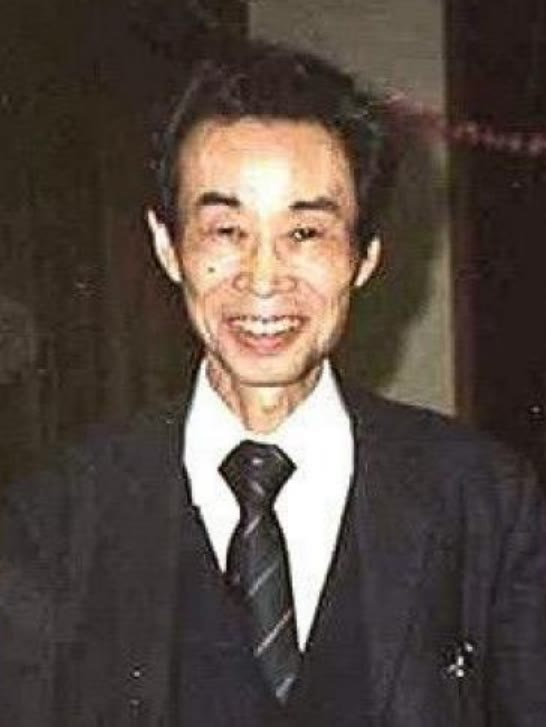
\includegraphics[width=0.34\linewidth]{images/book5/kimura.jpg}\hspace{0.05\linewidth}
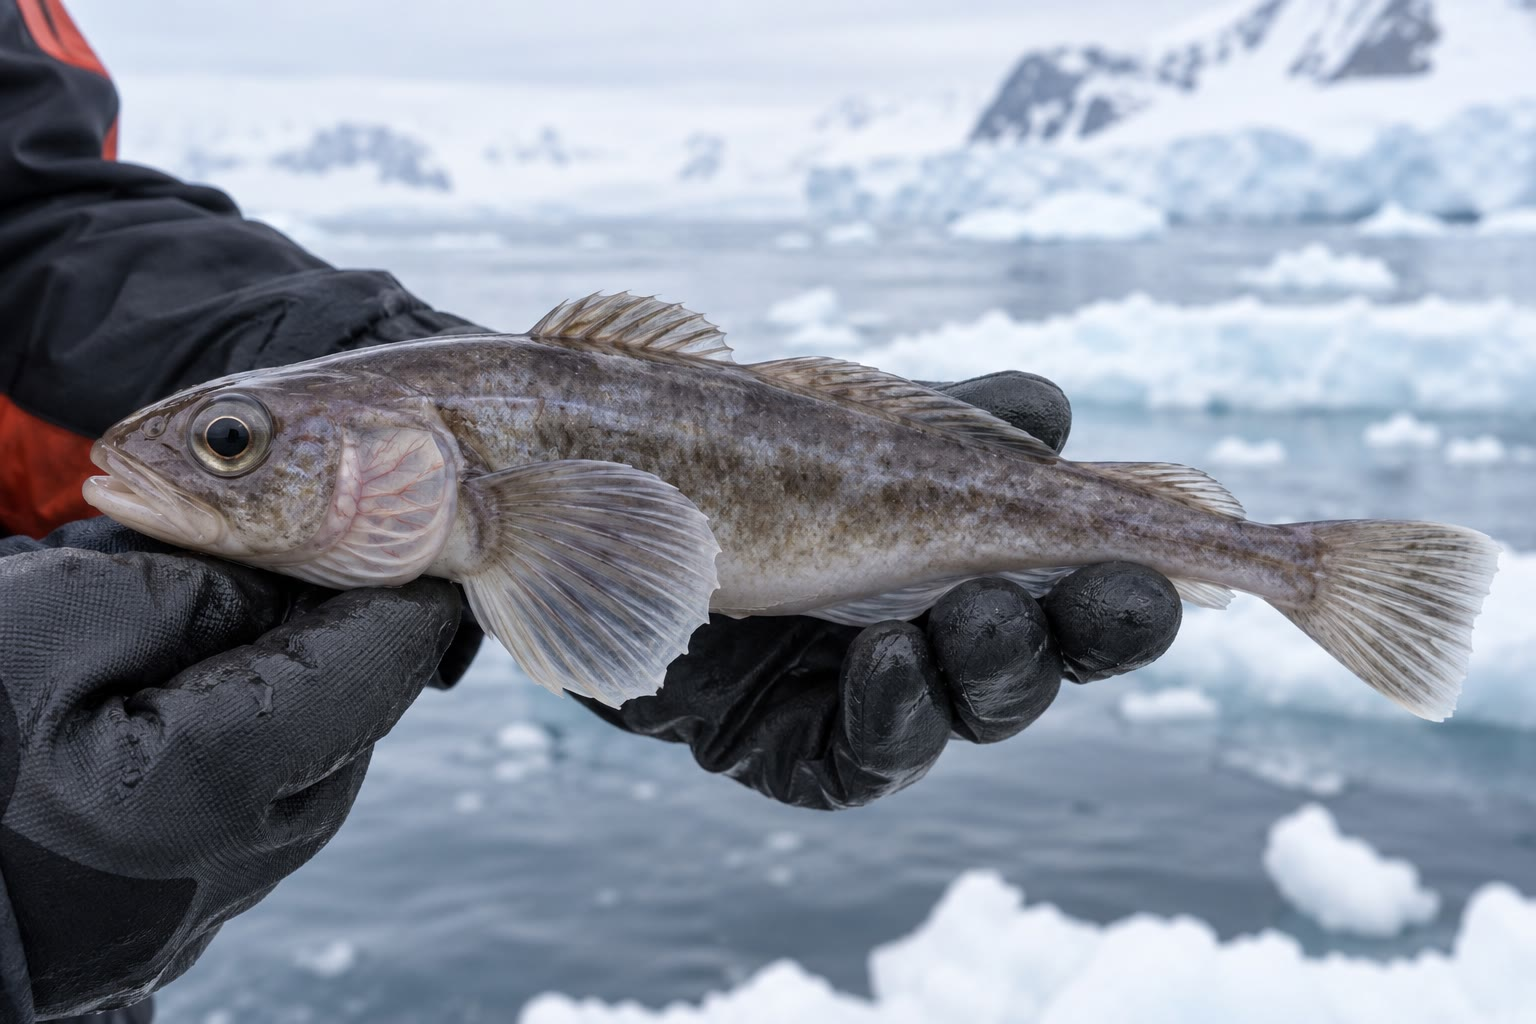
\includegraphics[width=0.5\linewidth]{images/book5/ai/b5-25-icefish.jpg}

{\small बाएँ: मोतू किमूरा (1924--1994), जिसने दिखाया कि अधिकांश आणविक
बदलाव संयोग से और उत्परिवर्तन-दर पर स्थिर होता है (छायाचित्र, 1986,
CC BY 4.0)। दाएँ: कोई अंटार्कटिक हिममीन, जिसका रक्त किसी प्रति-हिम
ग्लाइकोप्रोटीन से जमने से बचा रहता है, जो कोई एक करोड़ वर्ष पहले किसी
द्विगुणित पाचक-एंज़ाइम जीन और पुनरावृत्तियों की किसी शृंखला से जोड़ा
गया था।}
\end{omfigure}

\section{आणविक घड़ी}

\begin{proposition}[वह घड़ी और उसकी अनियमितताएँ]\label{prop:b3:molecular-evolution:clock}
\index{आणविक घड़ी}\index{अंशांकन}\index{दर-विषमता}\index{शिथिल घड़ी}\index{पीढ़ी-काल प्रभाव}
यदि प्रतिस्थापन प्रति स्थल प्रति वर्ष किसी अचर दर $k$ से उन दो
वंश-परंपराओं में जमा हों जो $T$ वर्ष पहले अलग हुई थीं, तो जिन स्थलों पर वे
भिन्न हैं उनका अंश, छोटे मानों के लिए, $d \approx 2kT$ है: यानी दो
अनुक्रमों का अपसरण कोई \emph{\omterm{prop:b3:molecular-evolution:clock}{आणविक घड़ी}} है (त्सुकरकांड्ल और पॉलिंग,
1965), जिसे किसी एक जीवाश्म-तिथि वाले विभाजन से \emph{अंशांकित} किया
जा सकता है और फिर उन विभाजनों के लिए पढ़ा जा सकता है जिनके कोई जीवाश्म
नहीं। वह घड़ी प्रसंभाव्य है --- कोई प्वासों प्रक्रम, इसलिए स्थलों की
किसी नियत संख्या भर $d$ का प्रसरण लगभग उसके माध्य के बराबर है --- और वह
तीन ज्ञात ढंगों से अनियमित है। हर प्रोटीन की अपनी दर है, जो उसके उन
स्थलों के अंश से तय होती है जिन्हें प्रकार्य बदलने देता है: प्रति स्थल
प्रति अरब वर्ष फ़ाइब्रिनोपेप्टाइड \num{8}, हीमोग्लोबिन
\num{1}, साइटोक्रोम~$c$ \num{0.3}, \omterm{def:b3:chromatin-epigenetics:nucleosome}{हिस्टोन}~H4 \num{0.01} प्रतिस्थापन।
वंश-परंपराओं के बीच दरें भिन्न हैं: चूँकि उदासीन दर प्रति पीढ़ी $\mu$
है, छोटी पीढ़ियों वाले प्राणी (कृंतक) लंबी पीढ़ियों वालों (नरवानर,
ह्वेल) से प्रति वर्ष अधिक बदलाव जमा करते हैं --- यानी \emph{\omterm{prop:b3:molecular-evolution:clock}{पीढ़ी-काल
प्रभाव}}, जिसकी आंशिक भरपाई इससे होती है कि प्रति-पीढ़ी उत्परिवर्तन-दरें
पीढ़ी की लंबाई के साथ चढ़ती हैं। और $d$ संतृप्त हो जाता है: एक बार अनेक
स्थल बदल जाने पर आगे के बदलाव उन्हीं स्थलों पर पड़ते हैं जो पहले ही बदल
चुके, इसलिए कच्चे अंतर को अनेक प्रहारों के लिए सुधारना पड़ता है, जैसा
\omterm{def:b3:bioinformatics:alignment}{संरेखण} वाले अध्याय की दूरियाँ करती हैं। आधुनिक \emph{\omterm{prop:b3:molecular-evolution:clock}{शिथिल घड़ियाँ}}
उस दर को किसी सांख्यिकीय प्रतिरूप के भीतर शाखा-दर-शाखा बदलने देती हैं
और एक साथ अनेक जीवाश्मों से अंशांकित होती हैं; वे मनुष्यों तथा
चिंपैंज़ियों के विभाजन की तिथि साठ से सत्तर लाख वर्ष रखती हैं, अपरायुक्त
स्तनी गणों की क्रिटेशस के अंत के पास, और प्राणियों तथा कवकों की
प्रीकैंब्रियन में, और उनकी दस से बीस प्रतिशत अनिश्चितताएँ अधिकांशतः उन
जीवाश्मों से आती हैं।
\end{proposition}
\begin{proof}
दोनों वंश-परंपराएँ प्रति स्थल $kT$ प्रतिस्थापन जमा करती हैं, इसलिए उनके
बीच का अंतर $2kT$ है, जहाँ स्थलों पर दो बार प्रहार न हुआ हो; और कोई
जीवाश्म-तिथि वाला जोड़ा $k = d/2T$ दे देता है। वह प्वासों प्रसरण तथा
प्रति-प्रोटीन दरें त्सुकरकांड्ल तथा पॉलिंग की, डिकरसन (1971) की और
किमूरा की कशेरुकी प्रोटीन-समुच्चयों पर फिट हैं; और वह संतृप्ति-सुधार
\omterm{def:b3:bioinformatics:alignment}{संरेखण} वाले अध्याय का जूक्स--कैंटर सूत्र है, $d_{\text{सत्य}} =
-\tfrac{3}{4}\ln(1 - \tfrac{4}{3}p)$। वंश-परंपराओं के बीच दर-विचरण
सापेक्ष-दर परीक्षणों से दिखाया गया: किसी बहिःसमूह $O$ और दो जातियों
$A$, $B$ के साथ, किसी कड़ी घड़ी के तहत दूरियाँ $d_{AO} - d_{BO}$ शून्य
होनी चाहिए, और नरवानरों के सामने कृंतकों के लिए वे नहीं हैं।
\end{proof}

\begin{omfigure}
\begin{tikzpicture}
\begin{axis}[
  width=0.68\linewidth, height=5.8cm,
  axis x line=bottom, axis y line=left,
  xmin=0, xmax=600, ymin=0, ymax=110,
  xlabel={अपसरण से बीता समय (करोड़ वर्ष)}, ylabel={प्रति 100 स्थल प्रतिस्थापन (सुधरे)},
  xlabel style={font=\small, at={(axis description cs:0.5,-0.12)}, anchor=north}, ylabel style={font=\small},
  tick label style={font=\small}, xtick={0,100,200,300,400,500,600}, ytick={0,20,40,60,80,100},
  clip=false,
]
\addplot[very thick, omThm, domain=0:130, samples=2] {2*0.4*x};
\addplot[very thick, omDef, domain=0:600, samples=2] {2*0.09*x};
\addplot[very thick, omMeth!70!black, domain=0:600, samples=2] {2*0.03*x};
\addplot[very thick, omProp!80!black, domain=0:600, samples=2] {2*0.001*x};
\addplot[only marks, mark=*, mark size=1.8pt, omDef] coordinates {(80,13) (100,20) (300,52) (400,75) (450,80)};
\addplot[only marks, mark=*, mark size=1.8pt, omMeth!70!black] coordinates {(80,4) (300,17) (450,29) (550,33)};
\addplot[only marks, mark=*, mark size=1.8pt, omThm] coordinates {(30,22) (80,68) (100,80)};
\node[font=\scriptsize, omThm, anchor=west] at (axis cs:132,104) {फ़ाइब्रिनोपेप्टाइड};
\node[font=\scriptsize, omDef, anchor=south east] at (axis cs:600,108) {हीमोग्लोबिन};
\node[font=\scriptsize, omMeth!70!black, anchor=north west] at (axis cs:530,35) {साइटोक्रोम $c$};
\node[font=\scriptsize, omProp!80!black, anchor=south east] at (axis cs:600,1.5) {हिस्टोन H4};
\end{axis}
\end{tikzpicture}

{\small \omterm{prop:b3:molecular-evolution:clock}{आणविक घड़ी}, प्रोटीन-दर-प्रोटीन। हर एक अपनी ही दर से चलती है, जो
इससे तय होती है कि उस अणु का कितना हिस्सा प्रकार्य बदलने के लिए स्वतंत्र
छोड़ता है: कोई फ़ाइब्रिनोपेप्टाइड, जो रक्त जमते समय काटकर फेंक दिया जाता
है, उस \omterm{def:b3:chromatin-epigenetics:nucleosome}{हिस्टोन} से सैकड़ों गुना तेज़ बदलता है जो DNA पैक करता है।}
\end{omfigure}

\section{अनुक्रमों में वरण पढ़ना}

\begin{definition}[dN/dS]\label{def:b3:molecular-evolution:dnds}
\index{पर्यायी प्रतिस्थापन}\index{अपर्यायी प्रतिस्थापन}\index{dN/dS अनुपात}\index{शोधक वरण}\index{धनात्मक वरण}
किसी प्रोटीन-कूटलेखी जीन में कोई प्रतिस्थापन \emph{पर्यायी} है यदि वह
उस ऐमीनो अम्ल को अपरिवर्तित छोड़े और \emph{अपर्यायी} यदि वह उसे बदल दे।
चूँकि आनुवंशिक कूट अधिकांश तीसरी स्थितियों को और कुछ पहली स्थितियों को
चुपचाप बदलने देता है, किसी सामान्य जीन के संभव उत्परिवर्तनों का लगभग
चौथाई पर्यायी है। मान लीजिए $d_{S}$ प्रति पर्यायी स्थल पर्यायी
प्रतिस्थापनों की संख्या है और $d_{N}$ प्रति अपर्यायी स्थल अपर्यायी
प्रतिस्थापन, और दोनों अनेक प्रहारों के लिए सुधरे हुए। पर्यायी बदलाव
उदासीन के पास हैं, इसलिए $d_{S}$ $2\mu T$ का आकलन करता है --- यानी वह
घड़ी; और वह अनुपात
\[
\omega = \frac{d_{N}}{d_{S}}
\]
नापता है कि वरण ने उस प्रोटीन का क्या किया है: $\omega = 1$ यदि
ऐमीनो-अम्ल बदलाव उतने ही स्वतंत्र हों जितने मौन बदलाव (कोई बंधन नहीं,
जैसा किसी \omterm{def:b3:molecular-evolution:duplication}{आभासी जीन} में); $\omega < 1$ \emph{शोधक वरण} के तहत, जिसमें
अधिकांश बदलाव हटा दिए जाते हैं --- किसी सामान्य जीन का
$\omega \approx 0.1$ से $0.2$ है, \omterm{def:b3:chromatin-epigenetics:nucleosome}{हिस्टोनों} का $0.001$; और
$\omega > 1$ \emph{धनात्मक वरण} के तहत, जिसमें ऐमीनो-अम्ल बदलावों का
पक्ष अकेले अपवाह की छूट से तेज़ी से लिया जाता है --- यानी MHC अणुओं की
प्रतिजन-बंधक खाँच, \omterm{def:b3:adaptive-immunity:antibody}{प्रतिरक्षियों} के साथ किसी होड़ में पड़े \omterm{def:b3:virology:virus}{विषाणुओं} के
पृष्ठ-प्रोटीन, निषेचन के शुक्राणु तथा अंड प्रोटीन, और रोमंथियों की
लाइसोज़ाइम, जिसे आमाशय में जीवाणु पचाने के लिए भर्ती किया गया।
किसी वृक्ष की किसी एक शाखा पर या स्थल-दर-स्थल गणित किया गया $\omega$
यह मानचित्रित कर देता है कि कोई प्रोटीन कहाँ और कब संयोग से नहीं बल्कि
वरण से बदला गया।
\end{definition}

\begin{omfigure}
\begin{tikzpicture}[every node/.style={font=\scriptsize}, >=stealth]
  \begin{axis}[
    width=0.52\linewidth, height=5.2cm,
    xbar, bar width=7pt, y=0.45cm,
    axis x line=bottom, axis y line=left,
    xmin=0.0005, xmax=5, xmode=log,
    xlabel={$\omega = d_{N}/d_{S}$},
    xlabel style={font=\small, at={(axis description cs:0.5,-0.12)}, anchor=north},
    symbolic y coords={histone H4, actin, insulin, typical gene, cytochrome $c$, pseudogene, ruminant lysozyme, MHC groove, HIV envelope},
    ytick=data, tick label style={font=\scriptsize},
    yticklabels={{हिस्टोन H4},{ऐक्टिन},{इंसुलिन},{सामान्य जीन},{साइटोक्रोम $c$},{आभासी जीन},{रोमंथी लाइसोज़ाइम},{MHC खाँच},{HIV परिवेष्टन}},
    yticklabels={{हिस्टोन H4},{ऐक्टिन},{इंसुलिन},{सामान्य जीन},{साइटोक्रोम $c$},{आभासी जीन},{रोमंथी लाइसोज़ाइम},{MHC खाँच},{HIV परिवेष्टन}},
    yticklabels={{हिस्टोन H4},{ऐक्टिन},{इंसुलिन},{सामान्य जीन},{साइटोक्रोम $c$},{आभासी जीन},{रोमंथी लाइसोज़ाइम},{MHC खाँच},{HIV परिवेष्टन}},
    xtick={0.001,0.01,0.1,1}, xticklabels={0.001,0.01,0.1,1},
    clip=false,
  ]
  \addplot[fill=omDef!50, draw=omDef] coordinates {(0.002,histone H4) (0.01,actin) (0.09,insulin) (0.15,typical gene) (0.05,cytochrome $c$) (1,pseudogene) (2.5,ruminant lysozyme) (3.5,MHC groove) (4,HIV envelope)};
  \draw[dashed, thick, omThm] (axis cs:1,histone H4) -- (axis cs:1,HIV envelope);
  \node[omThm, anchor=south, font=\tiny] at (axis cs:1,HIV envelope) {$\omega = 1$: उदासीन};
  \node[anchor=east, font=\tiny, gray] at (axis cs:0.5,actin) {शोधक};
  \node[anchor=west, font=\tiny, gray] at (axis cs:1.6,insulin) {धनात्मक};
  \end{axis}
\end{tikzpicture}

{\small $\omega$ की कोटियाँ। लगभग हर जीन एक से कहीं नीचे बैठा है, और
उसके ऐमीनो अम्ल \omterm{def:b3:molecular-evolution:dnds}{शोधक वरण} के पहरे में हैं; कोई \omterm{def:b3:molecular-evolution:duplication}{आभासी जीन} एक पर बहता है;
और जो थोड़े एक से ऊपर हैं वे होड़ों में पड़े या किसी नए काम पर हाल में
भर्ती हुए प्रोटीन हैं।}
\end{omfigure}

\begin{method}[$d_{N}/d_{S}$ का आकलन]\label{met:b3:molecular-evolution:method}
\index{कूटक-संरेखण}
(1) दोनों कूटलेखी अनुक्रम कूटक-दर-कूटक संरेखित कीजिए (उन प्रोटीनों को
संरेखित कीजिए, फिर DNA पर वापस मानचित्रित कीजिए, ताकि कोई अंतराल वह
पठन-खाँचा न तोड़े)। (2) हर कूटक के लिए पर्यायी तथा अपर्यायी \emph{स्थल}
गिनिए: उसकी तीनों स्थितियों में से हर एक को उन संभव बदलावों के अंश से
आँका जाता है जो मौन हैं --- कोई चौगुनी-अपह्रासी तीसरी स्थिति एक पर्यायी
स्थल गिनी जाती है, कोई ऐसी स्थिति जहाँ हर बदलाव उस ऐमीनो अम्ल को बदल दे
एक अपर्यायी स्थल, और कोई दुगुनी स्थिति एक का तिहाई और दूसरे का
दो-तिहाई। कूटकों भर जोड़िए: $S$ पर्यायी और $N$ अपर्यायी स्थल, जिनमें
$S + N = 3 \times$ कूटक। (3) उन अनुक्रमों के बीच पर्यायी तथा अपर्यायी
\emph{अंतर} गिनिए, और जो कूटक दो स्थितियों पर भिन्न हों उन्हें संभव
रास्तों पर औसत लेकर सुलझाइए। (4) $p_{S} = $ अंतर$/S$, $p_{N} = $ अंतर$/N$;
हर एक को अनेक प्रहारों के लिए जूक्स--कैंटर से सुधारिए। (5) $\omega =
d_{N}/d_{S}$; और $\omega \ne 1$ को उस प्रतिचयन-प्रसरण के सामने जाँचिए,
जो $d_{S}$ के छोटे होने पर बड़ा होता है --- दो निकट संबंधी अनुक्रम कोई
अविश्वसनीय अनुपात देते हैं, और दो बहुत दूर के अनुक्रमों का
$d_{S}$ संतृप्त होता है। (6) कहाँ और कब के लिए: किसी वृक्ष की हर शाखा
पर, या स्थल-वर्गों के किसी मिश्रण के साथ स्थल-दर-स्थल, $\omega$ फिट
कीजिए, और जाँचिए कि क्या $\omega > 1$ वाला कोई वर्ग उस फिट को बेहतर
करता है।
\end{method}

\section{पुराने जीनों से नए जीन}

\begin{definition}[द्विगुणन, कुल और अंतरण]\label{def:b3:molecular-evolution:duplication}
\index{जीन-द्विगुणन}\index{जीन-कुल}\index{नव-प्रकार्यन}\index{उप-प्रकार्यन}\index{आभासी जीन}\index{क्षैतिज जीन-अंतरण}
अधिकांश नए जीन पुरानों की प्रतियाँ हैं। कोई \emph{जीन-द्विगुणन} ---
असमान विनिमय से, प्रतिलोम-स्थानांतरण से, या पूरे जीनोम के दुगुने होने
से, जैसा कशेरुकियों के उद्गम पर दो बार हुआ और फिर अस्थिमीनों के पूर्वज
में तथा अनेक पादप वंश-परंपराओं में --- वहाँ दो \omterm{def:b3:genomics:comparative}{पैरालॉग} छोड़ जाता है
जहाँ एक था; और भिन्न जातियों के वे जीन जो किसी एक ही पुरखा जीन से उतरे
हों \omterm{def:b3:genomics:comparative}{ऑर्थोलॉग} हैं। उस प्रति का आम भवितव्य क्षय है: बंधन से छूटकर
($\omega \to 1$) वह कोई विराम-कूटक या कोई खाँचा-खिसकाव जमा कर लेती है
और कोई \emph{आभासी जीन} बन जाती है, जिनमें से मानव जीनोम कोई बीस हज़ार
ढोता है। कभी-कभी दोनों बच जाते हैं: \emph{नव-प्रकार्यन} से, जिसमें कोई
एक प्रति कोई नया प्रकार्य पा लेती है जबकि दूसरी पुराना रखे रहती है
(हिममीन का प्रति-हिम ग्लाइकोप्रोटीन, किसी ट्रिप्सिनोजन जीन से; नरवानरों
के लाल तथा हरे ऑप्सिन, चार करोड़ वर्ष पहले के उस द्विगुणन से जिसने वह
त्रिवर्णी दृष्टि दी जिसका वर्णन वर्ष~1 के खंड ने किया; और नेत्रोद
क्रिस्टलिन, उपापचयी एंज़ाइमों से); या \emph{उप-प्रकार्यन} से, जिसमें हर
प्रति उस पुरखे की अभिव्यक्ति या क्रियाशीलता का कुछ हिस्सा रखती है ताकि
दोनों ज़रूरी हों। बार-बार का द्विगुणन \emph{जीन-कुल} बना देता है ---
ग्लोबिन, परिवर्धन वाले अध्याय के Hox गुच्छे, किसी चूहे के हज़ार \omterm{def:b3:sensory-systems:chemical}{घ्राण
ग्राही} जीन, जिनका तिहाई मनुष्यों में आभासी जीन है। नए जीनों का दूसरा
स्रोत \emph{क्षैतिज अंतरण} है: जीवाणु असंबंधित जीवाणुओं से जीन
प्लास्मिडों, फ़ेजों तथा मुक्त DNA द्वारा पा लेते हैं, और इसी से किसी
अस्पताल में \omterm{def:b3:bacteriology:resistance}{प्रतिजैविक-प्रतिरोध} जातियाँ पार करता है और इसीलिए किसी
जीवाणु की ``जाति'' कोई क्रोड जीनोम है जिसे कोई खिसकता बादल घेरे है;
सुकेंद्रकियों में अंतरण बिरला है पर असली है --- वह \omterm{def:b3:genetic-engineering:plants}{T-DNA} जो
\emph{\omterm{def:b3:genetic-engineering:plants}{Agrobacterium}} पौधों में डालता है, ब्डेलॉइड रोटिफ़रों में
जीवाणु-जीन, और वे प्राचीन थोक अंतरण जो सूत्रकणिका तथा हरितलवक थे। जहाँ
अंतरण आम है वहाँ जीवन का इतिहास कोई जाल है, और किसी भी एक जीन से खींचा
गया वृक्ष उसी जीन का वृक्ष है।
\end{definition}

\begin{omfigure}
\begin{tikzpicture}[every node/.style={font=\scriptsize}, >=stealth]
  \node[draw, thick, rounded corners, fill=omDef!25, minimum width=1.8cm] (a) at (0,3) {पुरखा जीन};
  \node[draw, thick, rounded corners, fill=omDef!25, minimum width=1.2cm] (c1) at (-1.2,1.6) {प्रति 1};
  \node[draw, thick, rounded corners, fill=omDef!25, minimum width=1.2cm] (c2) at (1.2,1.6) {प्रति 2};
  \draw[->, thick] (a) -- (c1); \draw[->, thick] (a) -- (c2); \node[right, font=\tiny] at (0.9,2.4) {द्विगुणन};
  \node[draw, thick, rounded corners, fill=gray!20, align=center] (ps) at (-3.6,-0.2) {आभासी जीन\\$\omega \to 1$, फिर\\विराम-कूटक, क्षय};
  \node[draw, thick, rounded corners, fill=omThm!20, align=center] (neo) at (0,-0.2) {नव-प्रकार्यन\\एक प्रति नया काम लेती है\\(प्रति-हिम, लाल/हरा ऑप्सिन)};
  \node[draw, thick, rounded corners, fill=omMeth!25, align=center] (sub) at (3.9,-0.2) {उप-प्रकार्यन\\हर प्रति पुरानी अभिव्यक्ति\\का कुछ हिस्सा रखती है};
  \draw[->, thick] (c1.south) -- (ps.north); \draw[->, thick] (c2.south) -- (neo.north); \draw[->, thick] (c2.south) -- (sub.north);
  \node[right, align=left, font=\tiny] at (5.9,1.6) {सबसे आम भवितव्य: कुछ करोड़ वर्षों\\में लोप ($\sim$\num{20000}\\आभासी जीन मानव जीनोम में)};
  \node[right, align=left, font=\tiny] at (5.9,0.4) {बिरला: दोनों रखे जाते हैं, और कोई\\जीन-कुल बढ़ता है (ग्लोबिन, Hox,\\\num{1000} घ्राण ग्राही)};
  \node[right, align=left, font=\tiny] at (5.9,-0.8) {क्षैतिज अंतरण: कोई जीन\\किसी दूसरी जाति से आता है ---\\जीवाणुओं में रोज़ की बात};
\end{tikzpicture}

{\small किसी द्विगुणित जीन के भवितव्य। बंधन से छूटकर वह अतिरिक्त प्रति
प्रायः क्षय हो जाती है; कभी-कभी वरण उसे किसी नए प्रकार्य के लिए पकड़
लेता है, या दोनों प्रतियाँ पुराने को आपस में बाँट लेती हैं।}
\end{omfigure}

\begin{proof}[प्रमाण-सामग्री]
ओहनो (1970) ने द्विगुणन को नए जीनों का मुख्य स्रोत तब प्रस्तावित किया
जब कोई एक कुल भी अनुक्रमित नहीं हुआ था; ग्लोबिनों ने उसकी पुष्टि की, और
$\alpha$, $\beta$, $\gamma$, $\delta$, मायोग्लोबिन तथा पादप एवं जीवाणु
ग्लोबिनों का उनका वृक्ष द्विगुणन-तिथियों को कशेरुकी विकिरण से मिला
देता है। चेन, डिव्रीज़ और चेंग (1997) ने दिखाया कि हिममीन का प्रति-हिम
जीन अपना संकेत-अनुक्रम तथा पार्श्व अनुक्रम ट्रिप्सिनोजन से साझा करता है
और कि वे प्रति-हिम पुनरावृत्तियाँ किसी इंट्रॉन--एक्सॉन संधि पर फैले
किसी नौ-न्यूक्लियोटाइड टुकड़े के विस्तार से उठीं: यानी किसी पाचक
एंज़ाइम के फ़ालतू पुर्ज़ों से कोई नया प्रोटीन, जिसकी तिथि उस घड़ी ने
दक्षिणी महासागर के जमने पर रखी। थॉर्नटन और सहयोगियों (2006) ने
स्टेरॉइड ग्राहियों का पुरखा अनुक्रम फिर से खड़ा किया, उस पैंतालीस
करोड़ वर्ष पुराने प्रोटीन का संश्लेषण किया,
और पाया कि वह केवल एस्ट्रोजन पर अनुक्रिया देता था; और दो बाद के
प्रतिस्थापनों ने, जो पहचाने तथा जाँचे गए, उस द्विगुणित प्रति की पसंद
कॉर्टिसोल पर मोड़ दी --- यानी कोई पुनर्जीवित पुरखा, और उसके तथा उसके
वंशजों के बीच का रास्ता प्रयोगशाला में चलकर देखा गया।
\end{proof}

\section{जीन-वृक्ष और जाति-वृक्ष}

\begin{proposition}[अपूर्ण वंश-छँटाई]\label{prop:b3:molecular-evolution:ils}
\index{जीन-वृक्ष}\index{जाति-वृक्ष}\index{अपूर्ण वंश-छँटाई}\index{संगलन}\index{जातिवृत्तजीनोमिकी}
किसी जीन का वृक्ष उन जातियों के वृक्ष से मेल खाए, यह ज़रूरी नहीं जो उसे
ढोती हैं। \omterm{prop:b3:molecular-evolution:ils}{जाति-वृक्ष} $((A,B),C)$ वाली तीन जातियाँ लीजिए, जिनके
$A$--$B$ विभाजन से पहले आकार $N$ की कोई पुरखा समष्टि $T$ पीढ़ियों तक
बनी रही, इससे पहले कि वह $C$ से अलग हो। दो जीन-प्रतियाँ, एक $A$ से और एक $B$ से,
पीछे की ओर खोजने पर, किसी साझा पूर्वज में प्रति पीढ़ी दर $1/2N$ से
\emph{संगलित} होती हैं; और यह प्रायिकता कि वे तब तक संगलित नहीं हुईं जब
वे तीनों की पुरखा समष्टि में घुसें, $\mathrm{e}^{-T/2N}$ है, और फिर वे
तीनों वंश-रेखाएँ यादृच्छिक क्रम में संगलित होती हैं, इसलिए दो-तिहाई बार
वह \omterm{prop:b3:molecular-evolution:ils}{जीन-वृक्ष} $A$ या $B$ को $C$ के साथ जोड़ देता है। इसलिए यह प्रायिकता
कि वह \omterm{prop:b3:molecular-evolution:ils}{जीन-वृक्ष} उस \omterm{prop:b3:molecular-evolution:ils}{जाति-वृक्ष} से असहमत हो, है
\[
P_{\text{असंगत}} = \tfrac{2}{3}\,\mathrm{e}^{-T/2N} .
\]
मनुष्यों, चिंपैंज़ियों और गोरिल्लाओं के लिए, जिनका $T$ कुछ लाख पीढ़ियों
का है और $N$ \num{50000} के पास, जीनोम का लगभग तिहाई किसी ऐसे वृक्ष का
समर्थन करता है जिसमें मनुष्य गोरिल्लाओं के या चिंपैंज़ी गोरिल्लाओं के
उस \omterm{prop:b3:molecular-evolution:ils}{जाति-वृक्ष} से अधिक निकट हैं --- और यह देखा गया है। यही
\emph{\omterm{prop:b3:molecular-evolution:ils}{अपूर्ण वंश-छँटाई}}, द्विगुणन तथा लोप और क्षैतिज अंतरण के साथ, वह
कारण है कि \emph{जातिवृत्तजीनोमिकी} उस \omterm{prop:b3:molecular-evolution:ils}{जाति-वृक्ष} का अनुमान हज़ारों
\omterm{prop:b3:molecular-evolution:ils}{जीन-वृक्षों} से संगलन के किसी प्रतिरूप के तहत लगाती है, न कि उन्हें जोड़कर
कोई एक खींच देती है; वह उन पुरखा समष्टि-आकारों का आकलन भी असहमत वृक्षों
के अंश से करने देती है, और प्राचीन संकरण (आधुनिक मनुष्यों में
नियंडरथल DNA, भालुओं के बीच तथा तितलियों के बीच जीन-प्रवाह) उन वृक्षों
से पढ़ने देती है जो किसी ऐसी दिशा में असहमत हों जो अकेला अपवाह न बनाता।
\end{proposition}
\begin{proof}
$N$ की किसी द्विगुणित समष्टि में दो वंश-रेखाएँ हर पीढ़ी $2N$ प्रतियों
में से माता-पिता चुनती हैं और प्रायिकता $1/2N$ से कोई एक साझा करती हैं;
और $T$ पीढ़ियों भर कभी ऐसा न करने की संभावना $(1 - 1/2N)^{T} \approx
\mathrm{e}^{-T/2N}$ है। उस साझा पुरखा समष्टि में घुसती तीनों
वंश-रेखाएँ विनिमेय हैं, इसलिए सबसे पहले संगलित होता जोड़ा उन तीनों
जोड़ों में से हर एक प्रायिकता $1/3$ से होता है; और केवल जोड़ा $(A,B)$
उस \omterm{prop:b3:molecular-evolution:ils}{जाति-वृक्ष} से मेल खाता है, इसलिए इनमें से $2/3$ स्थितियाँ असहमत हैं।
न तो उस संगलन की दर और न वह विनिमेयता उस जीन पर निर्भर है, इसलिए वह
सूत्र हर उदासीन स्थल के लिए स्वतंत्र रूप से चलता है, और किसी जीनोम भर
असहमत वृक्षों का अंश $\mathrm{e}^{-T/2N}$ का आकलन कर देता है।
\end{proof}

\begin{omfigure}
\begin{tikzpicture}[every node/.style={font=\scriptsize}, >=stealth]
  % species tree as thick grey tubes
  \fill[gray!25] (0,0) -- (0.9,0) -- (2.8,4.2) -- (1.9,4.2) -- cycle;
  \fill[gray!25] (1.6,0) -- (2.5,0) -- (2.8,4.2) -- (1.9,4.2) -- cycle;
  \fill[gray!25] (2.35,2.6) -- (3.15,2.6) -- (3.15,0) -- (3.9,0) -- (3.9,3.4) -- (3.2,5.6) -- (2.3,5.6) -- (1.9,4.2) -- (2.8,4.2) -- cycle;
  \node[below] at (0.45,0) {A}; \node[below] at (2.05,0) {B}; \node[below] at (3.5,0) {C};
  \node[above left, font=\tiny, gray!70!black] at (1.0,4.2) {A--B विभाजन};
  \node[above left, font=\tiny, gray!70!black] at (1.0,5.6) {C से विभाजन};
  \draw[<->, gray!70!black] (-0.2,4.2) -- (-0.2,5.6) node[midway, left, font=\tiny, align=right] {$T$ पीढ़ियाँ,\\आकार $N$};
  \draw[gray!50, dashed] (-0.2,4.2) -- (1.9,4.2); \draw[gray!50, dashed] (-0.2,5.6) -- (2.3,5.6);
  % concordant gene lineages (blue)
  \draw[very thick, omDef] (0.4,0) -- (2.1,3.8) -- (2.2,4.0); \draw[very thick, omDef] (2.0,0) -- (2.2,4.0); \draw[very thick, omDef] (2.2,4.0) -- (2.6,5.0); \draw[very thick, omDef] (3.5,0) -- (2.6,5.0);
  \node[right, align=left, omDef] at (4.6,4.6) {नीला: A और B, C से विभाजन से\\पहले संगलित --- सहमत};
  % discordant lineages (red)
  \draw[very thick, omThm, dashed] (0.55,0) -- (2.35,4.2) -- (2.7,5.9); \draw[very thick, omThm, dashed] (2.15,0) -- (2.55,4.2) -- (2.9,5.3) -- (3.0,5.5); \draw[very thick, omThm, dashed] (3.65,0) -- (3.0,5.5); \draw[very thick, omThm, dashed] (3.0,5.5) -- (2.7,5.9);
  \node[right, align=left, omThm] at (4.6,3.2) {लाल: वे उस पुरखा समष्टि में संगलित\\नहीं हो पातीं (प्रायिकता\\$\mathrm{e}^{-T/2N}$), और फिर B पहले C से जुड़ती है:\\वह जीन-वृक्ष $((B,C),A)$ है};
  \node[right, align=left] at (4.6,1.4) {$P_{\text{असंगत}} = \tfrac{2}{3}\,\mathrm{e}^{-T/2N}$:\\$T = 2N$ के साथ, चार में एक जीन\\उस जाति-वृक्ष से असहमत};
\end{tikzpicture}

{\small किसी \omterm{prop:b3:molecular-evolution:ils}{जाति-वृक्ष} के भीतर \omterm{prop:b3:molecular-evolution:ils}{जीन-वृक्ष}। वे धूसर नलियाँ समष्टियाँ
हैं; और वे रेखाएँ किसी एक जीन की वंशावली। जो वंश-रेखाएँ उस छोटी पुरखा
समष्टि में नहीं मिल पातीं वे साथ-साथ गहरी वाली में घुसती हैं और
यादृच्छिक रूप से जोड़े बना लेती हैं --- इसलिए पास-पास पड़ी तीन जातियों
के जीनोम का तिहाई उन जातियों से भिन्न कहानी कहता है।}
\end{omfigure}

\begin{example}[किसी जीनोम का इतिहास पढ़ना]\label{ex:b3:molecular-evolution:cichlids}
विक्टोरिया झील की पाँच सौ सिक्लिड जातियाँ उन पंद्रह हज़ार वर्षों में
उठीं जब से वह झील फिर भरी --- यानी इतनी तेज़ी से कि उत्परिवर्तन उनके
बीच के अंतर जुटा ही न सकता। उनके जीनोम दिखाते हैं कि कैसे: जो प्रभेद
किसी तलभक्षी को किसी शैवाल-खुरचने वाले से अलग करते हैं वे उन नदी-मछलियों
में पहले से मौजूद विचरण के रूप में थे जिन्होंने उस झील को बसाया, और
छँटे तथा पुनर्संयोजित हुए, और वंश-परंपराओं के बीच के संकरण से बढ़े; उन
ऑप्सिन जीनों को साफ़ या गँदले पानी के लिए उन प्रतिस्थापनों से सुर में
किया गया जिन्हें उनकी शाखाओं का $\omega$ वरित दिखाता है; और वे
\omterm{prop:b3:molecular-evolution:ils}{जीन-वृक्ष} जीनोम भर एक-दूसरे से ठीक उसी ढर्रे में असहमत हैं जिसका
पूर्वानुमान \omterm{prop:b3:molecular-evolution:ils}{अपूर्ण वंश-छँटाई} तथा जीन-प्रवाह करते हैं। कोई विकिरण नए
जीनों का उद्गम नहीं बल्कि पुराने युग्मविकल्पियों का नए वरण के तहत नए
संयोजनों में पुनर्वितरण है --- जिसे वे अनुक्रम, युग्मविकल्पी-दर-युग्मविकल्पी,
दर्ज करते हैं, यदि कोई ऐसा वृक्ष पढ़ना जानता हो जो असल में कोई वन है।
\end{example}

\begin{omfigure}
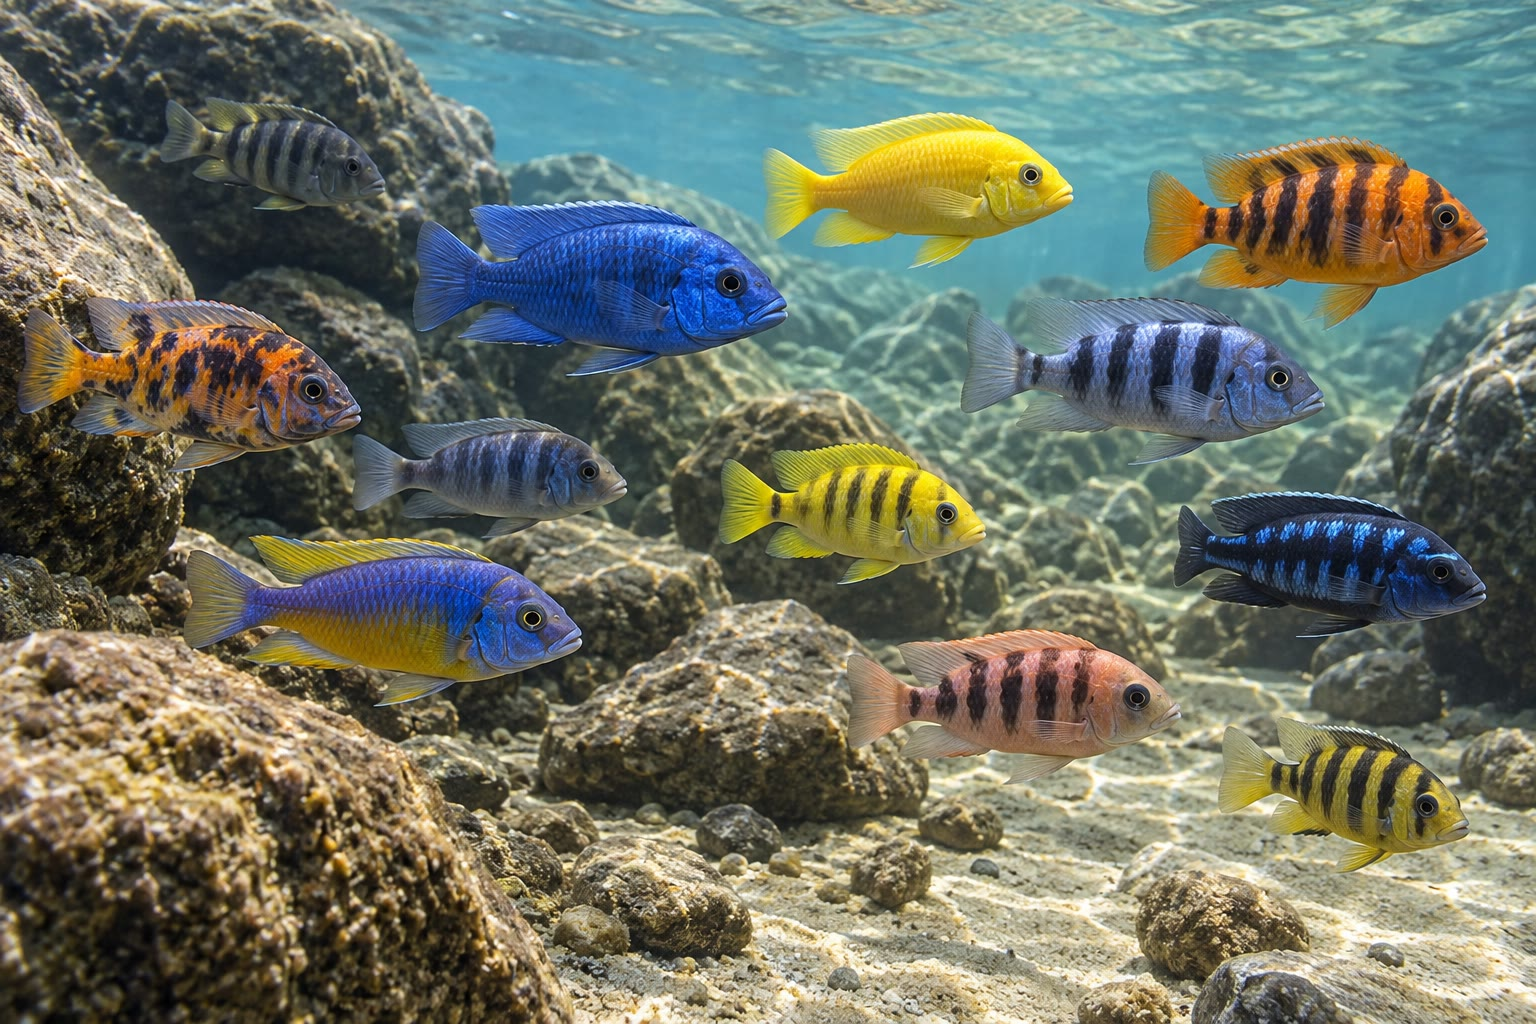
\includegraphics[width=0.6\linewidth]{images/book5/ai/b5-25-cichlids.jpg}

{\small किसी अफ़्रीकी झील के सिक्लिड: कुछ हज़ार वर्षों में सैकड़ों
जातियाँ, जिनके अंतर बड़े हिस्से में उसी विचरण से खींचे गए जो उनके साझा
पूर्वज पहले से ढो रहे थे।}
\end{omfigure}

\begin{remark}[आधार-रेखा के रूप में संयोग]\label{rem:b3:molecular-evolution:remark}
\omterm{thm:b3:molecular-evolution:neutral}{उदासीन सिद्धांत} यह दावा नहीं है कि वरण महत्वहीन है; वह इसका कथन है कि
जब वरण अनुपस्थित हो तब क्या होता है, और वह इतना परिशुद्ध है कि उसके
सामने जाँचा जा सके। चूँकि वह उदासीन दर उत्परिवर्तन-दर है, इसलिए अपसरण
समय नापता है; चूँकि उदासीन बदलाव उन स्थलों को भरता है जो वरण स्वतंत्र
छोड़ता है, इसलिए $\omega$ बंधन नापता है; और चूँकि उदासीन वंश-रेखाएँ
किसी ज्ञात दर से संगलित होती हैं, इसलिए \omterm{prop:b3:molecular-evolution:ils}{जीन-वृक्षों} की असहमति उन
समष्टियों का आकार नापती है जिन्हें किसी ने देखा ही नहीं। तब वरण वही है
जो संयोग घटा देने पर बचता है --- एक से ऊपर $\omega$ वाला कोई जीन, कोई
ऐसा झाड़ू जिसने किसी क्षेत्र से विचरण ख़ाली कर दिया हो, कोई ऐसा वृक्ष
जो किसी ऐसी दिशा में असहमत हो जिसकी व्याख्या अपवाह नहीं कर सकता।
अंटार्कटिक हिममीन का प्रति-हिम, रोमंथी की आमाशयी लाइसोज़ाइम, नरवानर का
तीसरा ऑप्सिन इसी तरह मिले अपवाद हैं, और हर एक किसी नक़ल किए गए जीन तथा
किसी नए काम की कहानी है। बाकी जीनोम कोई घड़ी है।
\end{remark}

\section{अभ्यास}

\begin{exercise}[$\star$]\label{exo:b3:molecular-evolution:1}
उदासीन \omterm{thm:b3:molecular-evolution:neutral}{प्रतिस्थापन दर} बताइए और शब्दों में समझाइए कि वह समष्टि-आकार पर
क्यों निर्भर नहीं है।
\end{exercise}

\begin{exercise}[$\star$]\label{exo:b3:molecular-evolution:2}
\omterm{def:b3:genomics:comparative}{ऑर्थोलॉग}, \omterm{def:b3:genomics:comparative}{पैरालॉग} और \omterm{def:b3:molecular-evolution:duplication}{आभासी जीन} परिभाषित कीजिए, और ग्लोबिन कुल से हर एक
का एक-एक उदाहरण दीजिए।
\end{exercise}

\begin{exercise}[$\star$]\label{exo:b3:molecular-evolution:3}
$\omega = d_{N}/d_{S}$ क्या नापता है? $\omega = 0.02$,
$\omega = 1.0$ और $\omega = 2.5$ की व्याख्या कीजिए, और हर तरह का एक-एक
जीन बताइए।
\end{exercise}

\begin{exercise}[$\star$]\label{exo:b3:molecular-evolution:4}
किमूरा ने यह निष्कर्ष क्यों निकाला कि अधिकांश प्रतिस्थापन उदासीन हैं?
वह तर्क अध्याय के आरंभ की संख्याओं के साथ फिर कहिए।
\end{exercise}

\begin{exercise}[$\star\star$]\label{exo:b3:molecular-evolution:5}
$N = 5000$। किमूरा के सूत्र से $s
= 0$, $s = 0.001$, $s = 0.01$ और $s = -0.001$ वाले किसी नए उत्परिवर्तन
की \omterm{thm:b3:molecular-evolution:neutral}{स्थिरण प्रायिकता} निकालिए, और टिप्पणी कीजिए कि कौन-से प्रभावतः उदासीन
हैं।
\end{exercise}

\begin{exercise}[$\star\star$]\label{exo:b3:molecular-evolution:6}
दो जातियाँ किसी ऐसे जीन के \qty{12}{\%} स्थलों पर भिन्न हैं जिसकी
उदासीन दर प्रति स्थल प्रति वर्ष \qty{2e-9}{} है। जूक्स--कैंटर सुधार के
साथ और उसके बिना उनका अपसरण-काल आँकिए। किस कच्चे अंतर पर वह सुधार दो का
गुणक छू लेता है?
\end{exercise}

\begin{exercise}[$\star\star$]\label{exo:b3:molecular-evolution:7}
300 कूटकों के किसी जीन के 700 अपर्यायी और 200 पर्यायी स्थल हैं। दो
जातियों के बीच वह 7 अपर्यायी और 10 पर्यायी अंतर दिखाता है। $p_{N}$,
$p_{S}$ और $\omega$ निकालिए (बिना सुधार)। कौन-सा वरण-शासन? और यदि वे
गिनतियाँ 35 तथा 10 होतीं तो?
\end{exercise}

\begin{exercise}[$\star\star$]\label{exo:b3:molecular-evolution:8}
मानव और चिंपैंज़ी के उदासीन अनुक्रम \qty{1.2}{\%} स्थलों पर भिन्न हैं;
वह विभाजन \qty{6.5}{Myr} पहले था, और पीढ़ी-काल \qty{25}{yr}। प्रति स्थल
प्रति पीढ़ी उत्परिवर्तन-दर आँकिए, और $6\times 10^{9}$ क्षारों के किसी
द्विगुणित जीनोम में हर पीढ़ी नए उत्परिवर्तनों की संख्या।
\end{exercise}

\begin{exercise}[$\star\star$]\label{exo:b3:molecular-evolution:9}
$N = \num{50000}$ और दोनों विभाजनों के बीच $T = \num{100000}$ पीढ़ियों
के साथ, मानव, चिंपैंज़ी तथा गोरिल्ला के लिए \omterm{prop:b3:molecular-evolution:ils}{जाति-वृक्ष} से असहमत
\omterm{prop:b3:molecular-evolution:ils}{जीन-वृक्षों} का अंश निकालिए। कौन-सा $T$ उसे \qty{10}{\%} कर देता?
\end{exercise}

\begin{exercise}[$\star\star\star$]\label{exo:b3:molecular-evolution:10}
दिखाइए कि किमूरा का सूत्र $1/2N$ तक घट जाता है जब $s \to 0$, और
$2s$ तक जब $4Ns \gg 1$, और यह कि $s < 0$ के लिए, जिसमें $4N|s| \gg 1$ हो, वह
$2|s|\,\mathrm{e}^{-4N|s|}$ जैसा बरताव करता है। फिर आँकिए कि $10^{4}$ की
किसी समष्टि में किसी उत्परिवर्तन को कितना हानिकारक होना पड़ेगा कि उसकी
\omterm{thm:b3:molecular-evolution:neutral}{स्थिरण प्रायिकता} उदासीन से सौ गुना नीचे आ जाए।
\end{exercise}

\begin{exercise}[$\star\star\star$]\label{exo:b3:molecular-evolution:11}
कोई सापेक्ष-दर परीक्षण: कोई बहिःसमूह $O$ चूहे से सुधरी दूरी $0.30$ पर
है और मनुष्य से $0.24$ पर, और चूहा तथा मनुष्य $0.20$ की दूरी पर। उनके
विभाजन से चूहे तथा मनुष्य की शाखा-लंबाइयाँ निकालिए (मानिए कि वह
विभाजन-बिंदु दोनों रास्तों पर $O$ से समदूरस्थ है), और उनका अनुपात।
\qty{0.5}{yr} की चूहा-पीढ़ी और \qty{25}{yr} की मानव-पीढ़ी के साथ, कोई
कड़ी प्रति-पीढ़ी घड़ी उस अनुपात के लिए क्या पूर्वानुमान करती, और वह
प्रेक्षण प्रति-पीढ़ी उत्परिवर्तन-दरों के बारे में क्या कहता है?
\end{exercise}

\begin{exercise}[$\star\star\star$]\label{exo:b3:molecular-evolution:12}
कोई द्विगुणित जीन बंधन से छूट जाता है ($\omega = 1$), उदासीन दर
$k = \qty{2e-9}{}$ प्रति स्थल प्रति वर्ष पर। 1000 क्षारों के किसी कूटलेखी
अनुक्रम में, पहले विराम-कूटक या खाँचा-खिसकाव तक मोटे तौर पर कितने वर्ष
प्रत्याशित हैं (मानिए कि किसी कूटलेखी अनुक्रम में यादृच्छिक बिंदु
उत्परिवर्तनों का लगभग \qty{4}{\%} कोई विराम-कूटक बनाता है, और
अंतर्वेशन-विलोपन छोड़ दीजिए)? उस समय से तुलना कीजिए जो वरण के पास कोई
नया प्रकार्य ढूँढ़ने को है, और समझाइए कि अधिकांश प्रतियाँ क्यों मर जाती हैं।
\end{exercise}

\section{समस्या: बदलाव की दर}

\begin{problem}[{सप्तांत समस्या --- संख्याओं में किसी जीनोम का इतिहास:
मानव--चिंपैंज़ी अपसरण से उत्परिवर्तन-दर, किमूरा का प्रतिस्थापन-भार,
वरित उत्परिवर्तनों की स्थिरण-संभावनाएँ, कूटक-गिनतियों से किसी जीन का
$\omega$, किसी द्विगुणन के लिए पढ़ी गई घड़ी, और महाकपियों के बीच
जीन-वृक्षों की असहमति, जिसका अंत उत्परिवर्तन-दर पर होता है, उस जीन के
$\omega$ पर, और असहमत अंश पर}]
\label{pb:b3:molecular-evolution:1}
आँकड़े: मानव--चिंपैंज़ी उदासीन अपसरण $d = 0.012$; विभाजन
\qty{6.5}{Myr} पहले; पीढ़ी \qty{25}{yr}; द्विगुणित जीनोम $6\times
10^{9}$ क्षार, \qty{1.5}{\%} कूटलेखी। पुरखा समष्टि $N =
\num{50000}$। जीन: 400 कूटक, 920 अपर्यायी और 280 पर्यायी
स्थल; मानव--चूहा अंतर 46 अपर्यायी और 84 पर्यायी।
मानव--चूहा विभाजन \qty{90}{Myr}। ग्लोबिन: $\alpha$ और $\beta$
ऐमीनो-अम्ल स्थलों के \qty{55}{\%} पर भिन्न (कच्चा); हीमोग्लोबिन की दर
प्रति स्थल प्रति वर्ष \num{1e-9}। महाकपि: गोरिल्ला तथा चिंपैंज़ी
विभाजनों के बीच $T$ \num{80000} पीढ़ियाँ। हाल्डेन की सीमा: प्रति
300 पीढ़ियाँ एक वरित प्रतिस्थापन।

\medskip
\noindent\textbf{भाग I --- वह दर।}
\begin{enumerate}
  \item $d = 2kT$ से, $k$ प्रति स्थल प्रति वर्ष निकालिए, फिर $\mu$
        प्रति स्थल प्रति पीढ़ी।
  \item प्रति द्विगुणित जीनोम प्रति पीढ़ी नए उत्परिवर्तन, और उनमें से
        कितने कूटलेखी अनुक्रम में पड़ते हैं।
  \item उदासीन दर पर पूरे जीनोम में प्रति पीढ़ी स्थिर हुए प्रतिस्थापन
        (वह समष्टि प्रति स्थल प्रति पीढ़ी $\mu$ स्थिर करती है)।
        हाल्डेन की सीमा से तुलना कीजिए और किमूरा का निष्कर्ष निकालिए।
  \item $N = \num{50000}$ की किसी समष्टि में, पूरी समष्टि में प्रति
        स्थल प्रति पीढ़ी कितने नए उदासीन उत्परिवर्तन उठते हैं, और उनका
        कितना अंश कभी स्थिर होगा?
  \item जिस उदासीन उत्परिवर्तन को स्थिर होना है उसे कितना समय लगता है,
        पीढ़ियों तथा वर्षों में? मानव--चिंपैंज़ी विभाजन से बीते समय से
        तुलना कीजिए।
  \item समझाइए कि प्रश्न~5 के बावजूद दो जातियों का अपसरण उनके विभाजन
        से बीता समय क्यों नापता है, न कि वह समय जब से उनके युग्मविकल्पी
        स्थिर हुए।
\end{enumerate}

\medskip
\noindent\textbf{भाग II --- वरण की संभावनाएँ।}
\begin{enumerate}[resume]
  \item $N = \num{50000}$ में किसी उदासीन उत्परिवर्तन की, और $s = 0.001$,
        $s = 0.01$, $s = 0.1$ वालों की \omterm{thm:b3:molecular-evolution:neutral}{स्थिरण प्रायिकता}।
  \item किस $s$ के लिए $4Ns = 1$ है? उस सीमा की व्याख्या कीजिए।
  \item $s = -0.001$ वाला कोई हानिकारक उत्परिवर्तन: उदासीन के सापेक्ष
        \omterm{thm:b3:molecular-evolution:neutral}{स्थिरण प्रायिकता}। और $s = -10^{-5}$?
  \item यदि किसी जीन के नए उत्परिवर्तनों का अंश $10^{-5}$ $s = 0.01$ के
        साथ लाभकारी हो और बाकी उदासीन, तो उस जीन के प्रतिस्थापनों का
        कितना अंश अनुकूली है? टिप्पणी कीजिए कि वरण काम करते हुए भी उस
        अनुक्रम में कितनी बिरली बार दिखता है।
  \item मानव--चूहा जीन के लिए $p_{N}$ तथा $p_{S}$ निकालिए, हर एक को
        जूक्स--कैंटर से सुधारिए, और $\omega$ दीजिए।
  \item $\omega$ की व्याख्या कीजिए; और उस विभाजन-काल से उस उदासीन दर का
        आकलन कीजिए जो उस जीन का $d_{S}$ माँगता है (प्रति स्थल प्रति
        वर्ष)। क्या वह प्रश्न~1 से संगत है?
\end{enumerate}

\medskip
\noindent\textbf{भाग III --- घड़ियाँ और प्रतियाँ।}
\begin{enumerate}[resume]
  \item $\alpha$--$\beta$ ग्लोबिन के अंतर को अनेक प्रहारों के लिए
        सुधारिए ($d = -\ln(1 - p)$ काम में लीजिए, यानी अनेक अवस्थाओं
        वाला प्रोटीन संस्करण), और हीमोग्लोबिन की दर से उस द्विगुणन की
        तिथि निकालिए।
  \item वह तिथि जबड़ेवाले कशेरुकियों के उद्गम के पास पड़ती है
        (\qtyrange{450}{500}{Myr})। अलग-अलग $\alpha$ तथा $\beta$
        शृंखलाएँ होना वह क्या करने देता है जो कोई एक शृंखला नहीं करने
        देती?
  \item फ़ाइब्रिनोपेप्टाइड प्रति स्थल प्रति वर्ष $8\times 10^{-9}$ से
        बदलते हैं। दो जातियाँ \qty{40}{Myr} पहले अलग हुईं: प्रत्याशित
        कच्चा अंतर? यह प्रोटीन \qty{500}{Myr} के विभाजनों की तिथि
        निकालने के लिए बेकार क्यों है?
  \item \omterm{def:b3:chromatin-epigenetics:nucleosome}{हिस्टोन} H4 $10^{-11}$ से बदलता है: \qty{1000}{Myr} भर 100
        स्थलों में कितने प्रतिस्थापन? वह हाल के विभाजनों के लिए बेकार
        क्यों है?
  \item कोई द्विगुणित जीन द्विगुणन के क्षण से $\omega = 1$ के साथ बहता
        है। यदि कूटलेखी अनुक्रम के \qty{4}{\%} प्रतिस्थापन विराम बनाएँ,
        और उस जीन के 1200 स्थल प्रति स्थल प्रति वर्ष $2\times
        10^{-9}$ की दर पर हों, तो पहले विराम-कूटक तक का प्रत्याशित समय
        आँकिए।
  \item पूरे-जीनोम द्विगुणन किसी एक ही अनुवर्ती द्विगुणन से प्रतियों को
        बचने की बेहतर संभावना क्यों देता है?
\end{enumerate}

\medskip
\noindent\textbf{भाग IV --- वृक्षों के भीतर वृक्ष।}
\begin{enumerate}[resume]
  \item यह प्रायिकता कि गोरिल्ला-विभाजन से पहले की \num{80000}
        पीढ़ियों में कोई मानव तथा कोई चिंपैंज़ी वंश-रेखा संगलित न हो।
  \item \omterm{prop:b3:molecular-evolution:ils}{जाति-वृक्ष} से असहमत \omterm{prop:b3:molecular-evolution:ils}{जीन-वृक्षों} का अंश। देखा गया: लगभग
        \qty{30}{\%}। संगत?
  \item असहमत वृक्षों में से कितना अंश मनुष्य को गोरिल्ला के साथ जोड़ता
        है, और कितना चिंपैंज़ी को गोरिल्ला के साथ? बराबरी से कोई प्रबल
        विचलन क्या दिखाता?
  \item यदि वह पुरखा समष्टि $N = \num{10000}$ की होती, तो आप कौन-सा
        असहमत अंश प्रत्याशित करते? इसलिए देखा गया अंश हमारे पूर्वजों की
        संख्याओं के बारे में क्या कहता है?
  \item हज़ार जीनों को किसी एक \omterm{def:b3:bioinformatics:alignment}{संरेखण} में जोड़ देना कोई आश्वस्त पर शायद
        ग़लत वृक्ष क्यों देता है, और कोई संगलन-विधि इसके बजाय क्या करती
        है?
  \item ग़ैर-अफ़्रीकी मनुष्यों में नियंडरथल DNA लगभग \qty{2}{\%} है और
        उसे ढोते वृक्ष कुछ यूरोपीयों को नियंडरथलों के साथ अफ़्रीकियों से
        अधिक बार जोड़ते हैं। यह \omterm{prop:b3:molecular-evolution:ils}{अपूर्ण वंश-छँटाई} क्यों नहीं है?
  \item सारांश दीजिए: $\mu$ (प्रश्न~1), उस जीन का $\omega$
        (प्रश्न~11), और असहमत अंश (प्रश्न~20)।
\end{enumerate}
\end{problem}
